\documentclass{article}
\usepackage{amsmath}
\usepackage{tikz}
\usetikzlibrary{matrix}

\begin{document}

\begin{figure}[h]
    \centering
    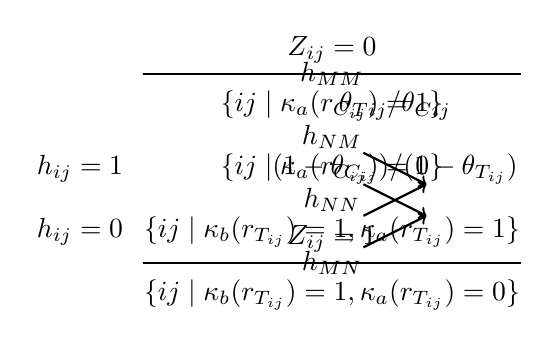
\begin{tikzpicture}[scale=0.8]
        % Define coordinates for the nodes
        \coordinate (A) at (0,0);
        \coordinate (B) at (6,0);
        \coordinate (C) at (0,3);
        \coordinate (D) at (6,3);
        
        % Draw the rectangles
        \draw[thick] (A) rectangle (B) node[midway, above] {$Z_{ij}=1$};
        \draw[thick] (C) rectangle (D) node[midway, above] {$Z_{ij}=0$};
        
        % Draw the horizontal lines
        \draw[thick] (A |- C) -- (B |- D);
        \draw[thick] (A |- D) -- (B |- C);
        
        % Draw the vertical lines
        \draw[thick] (A -| B) -- (A -| D);
        \draw[thick] (B -| A) -- (B -| D);
        
        % Add labels for the conditions
        \node at (3,-0.5) {$\{ij\mid\kappa_b(r_{T_{ij}})=1,\kappa_a(r_{T_{ij}})=0\}$};
        \node at (3,0.5) {$\{ij\mid\kappa_b(r_{T_{ij}})=1,\kappa_a(r_{T_{ij}})=1\}$};
        \node at (3,2.5) {$\{ij\mid\kappa_a(r_{C_{ij}})=1\}$};
        \node at (3,1.5) {$\{ij\mid\kappa_a(r_{C_{ij}})=0\}$};
        
        % Add the expected values
        \node at (3,1) {$h_{NN}$};
        \node at (3,0) {$h_{MN}$};
        \node at (3,2) {$h_{NM}$};
        \node at (3,3) {$h_{MM}$};
        
        % Add the labels for the treatment status
        \node at (-1,1.5) {$h_{ij}=1$};
        \node at (-1,0.5) {$h_{ij}=0$};
        
        % Add the legend
        \node at (4,2.5) {$\theta_{Tij}/\theta_{Cij}$};
        \node at (4,1.5) {$(1-\theta_{C_{ij}})/(1-\theta_{T_{ij}})$};
        
        % Add the arrows
        \draw[->, thick] (3.5,1.75) -- (4.5,1.25);
        \draw[->, thick] (3.5,0.75) -- (4.5,1.25);
        \draw[->, thick] (3.5,0.25) -- (4.5,0.75);
        \draw[->, thick] (3.5,1.25) -- (4.5,0.75);
    \end{tikzpicture}
    \caption{An illustration of how the cases are moved by the treatment in case$^2$-studies, within the stratum defined by levels of $(x_{ij},u_{ij})$ in which $\theta_{Tij}/\theta_{Cij}$ and $(1-\theta_{C_{ij}})/(1-\theta_{T_{ij}})$ are the largest. The left panel is the case allocation when all are treated, and the right panel is the case allocation when all the subjects are untreated. The numbers $h_{NN}, h_{MN}, h_{NM}, h_{MM}$ are expected values.}
    \label{fig:case2_study}
\end{figure}

\end{document}